\documentclass[11pt]{article}
\usepackage[scaled=0.92]{helvet}
\usepackage{geometry}
\geometry{letterpaper,tmargin=1in,bmargin=1in,lmargin=1in,rmargin=1in}
\usepackage[parfill]{parskip} % Activate to begin paragraphs with an empty line rather than an indent %\usepackage{graphicx}
\usepackage{amsmath,amssymb, mathrsfs,  mathtools, dsfont}
\usepackage{tabularx}
\usepackage{tikz-cd}
\usepackage[font=footnotesize,labelfont=bf]{caption}
\usepackage{graphicx}
\usepackage{xcolor}
%\usepackage[linkbordercolor ={1 1 1} ]{hyperref}
%\usepackage[sf]{titlesec}
\usepackage{natbib}
%\usepackage{tikz-cd}

\usepackage{../../Tianpei_Report}

%\usepackage{appendix}
%\usepackage{algorithm}
%\usepackage{algorithmic}

%\renewcommand{\algorithmicrequire}{\textbf{Input:}}
%\renewcommand{\algorithmicensure}{\textbf{Output:}}



\begin{document}
\title{Lecture 5: K-Nearest Neigbhor Rules}
\author{ Tianpei Xie}
\date{ Dec. 19th., 2022 }
\maketitle
\tableofcontents
\newpage
\section{Nearest Neighbor Rules}
\subsection{The Classification Rule}
\begin{itemize}
\item \begin{definition} (\emph{\textbf{Nearest Neighbor Rules}})\\
Formally, we define \underline{\emph{\textbf{the $k$-NN rule}}} by
\begin{align*}
g_n(x) &= \left\{\begin{array}{cc}
1 & \sum_{i=1}^{n}w_{n,i}\ind{Y_i = 1} > \sum_{i=1}^{n}w_{n,i}\ind{Y_i = 0}\\
0 & \text{o.w.}
\end{array}
\right.
\end{align*} where $w_{n,i} = 1/ k$ if $X_i$ is among the \emph{\textbf{$k$ nearest neighbors}} of $x$, and $w_{n,i} = 0$ elsewhere. 

$X_i$ is said to be \emph{\textbf{the $k$-th nearest neighbor}} of $x$ if the distance $d(x,X_i)$ is the \emph{$k$-th smallest} among $d(x,X_1), \xdotx{,} d(x,X_n)$  In case of a \emph{distance tie}, the candidate with the smaller index is said to be closer to $x$. The decision is based upon a \emph{\textbf{majority vote}}. It is convenient to let $k$ be \emph{odd}, to avoid voting ties. 
\end{definition}

\item \begin{remark} (\emph{\textbf{Voronoi Partition}}) \\
At every point the decision is the label ofthe \emph{closest} data point. \emph{The set of points whose nearest neighbor is $X_i$} is called \emph{\textbf{\underline{the Voronoi cell}} of $X_i$}. The partition induced by \emph{the Voronoi cells} is a \underline{\emph{\textbf{Voronoi partition}}}.   
\end{remark}


\begin{figure}
\begin{minipage}[t]{1\linewidth}
  \centering
  \centerline{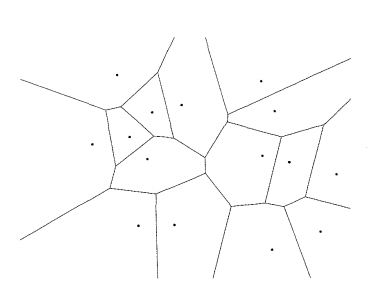
\includegraphics[scale = 0.6]{knn_voronoi_set.png}}
\end{minipage}
\caption{\footnotesize{\textbf{Varona partition of K-NN rules \citep{devroye2013probabilistic}. }}}
\label{fig: knn_voronoi_set}
\end{figure}

\item \begin{remark} (\emph{\textbf{Ordered Statistic}})\\
We fix $x \in \bR^d$, and \emph{\textbf{reorder}} the data $(X_1, Y_1) \xdotx{,} (X_n , Y_n)$ according to \emph{\textbf{increasing values}} of $d(x, X_i)$. The \emph{reordered data sequence} is denoted by
\begin{align*}
(X_{(1)}(x), Y_{(1)}(x)) \xdotx{,} (X_{(n)}(x), Y_{(n)}(x)) 
\end{align*} where $X_{(k)}(x)$ is the $k$-th nearest neighbor of $x$. For short, we write it as $(X_{(k)}, Y_{(k)})$.
\end{remark}
\end{itemize}


\section{Consistency}
\subsection{Asymptotic Consistency}
\begin{itemize}
\item \begin{definition}
Denote \emph{the probability measure} for $X$ by $\cP_{X}$ and let $B_{x, \epsilon}$ be the \emph{\textbf{closed ball}} centered at $x$ of radius $\epsilon > 0$. The collection of all $x$ with $\cP_{X}(B_{x ,\epsilon}) > 0$ \emph{for all} $\epsilon > 0$ is called \emph{\textbf{the support} of $X$} or $\cP_{X}$.
\end{definition}

\item \begin{lemma}\citep{devroye2013probabilistic}\\
If $x \in \text{support}(\cP_{X})$ and $\lim\limits_{n\rightarrow \infty}k/n = 0$, then 
\begin{align*}
d(x,X_{(k)}(x)) \rightarrow 0, \quad a.s.
\end{align*} 
If $X$ is independent of the data and has probability measure $\cP_{X}$, then 
\begin{align*}
d(X, X_{(k)}(x)) \rightarrow 0, \quad a.s.
\end{align*}   whenever $k/n \rightarrow 0$.
\end{lemma}
\end{itemize}

\subsection{Stone's Lemma}
\begin{itemize}
\item 
\begin{lemma} (\textbf{Stone's Lemma})  \citep{devroye2013probabilistic}\\
For any integrable function $f$, any $n$, and any $k \le n$:
\begin{align}
\sum_{i=1}^{k}\E{}{\abs{f\paren{X_{(i)}(X)}}} &\le k \gamma_d \E{}{\abs{f(X)}}, \label{eqn: stone_lemma}
\end{align}
where $\gamma_d \le \paren{1+ 2/\sqrt{2 - \sqrt{3}}}^d - 1$ depends upon the \textbf{dimension} only.
\end{lemma}

\item \begin{lemma} (\textbf{Approximation with K-NN})  \citep{devroye2013probabilistic}\\
For any integrable function $f$,
\begin{align*}
\frac{1}{k}\sum_{i=1}^{k}\E{}{\abs{f(X) - f\paren{X_{(i)}(X)}}} \to 0
\end{align*} as $n \rightarrow \infty$ whenever $k/n \rightarrow 0$.
\end{lemma}
\end{itemize}

\subsection{The Asymptotic Probability of Error}

\subsection{Stone's Theorem}
\begin{itemize}
\item \begin{remark} (\emph{\textbf{Estimate Posterior Conditional Probability with Weighted Averages}})\\
Consider a rule based on an estimate of the a \emph{\textbf{posteriori probability}} $\eta$ of the form
\begin{align*}
\eta_n(x) &= \sum_{i=1}^{n}\ind{Y_i = 1}W_{n,i}(x) = \sum_{i=1}^{n}Y_i \,W_{n,i}(x)
\end{align*}
where the weights $W_{n,i}(x) = W_{n,i}(x, X_1 \xdotx{,} X_n)$ are nonnegative and sum to one:
\begin{align*}
\sum_{i=1}^{n}W_{n,i}(x)  = 1.
\end{align*} $\eta_n$ is a \underline{\emph{\textbf{weighted average estimator}}} of $\eta$. 

The \emph{\textbf{classification rule}} is defined as
\begin{align*}
g_n(x) &= \left\{\begin{array}{cc}
0 &  \sum_{i=1}^{n}\ind{Y_i = 1}W_{n,i}(x)  \le \sum_{i=1}^{n}\ind{Y_i = 0}W_{n,i}(x)  \\
1 & \text{o.w.}
\end{array}
\right. \\
&=  \left\{\begin{array}{cc}
0 &   \sum_{i=1}^{n}Y_i \,W_{n,i}(x) \le \frac{1}{2}  \\
1 & \text{o.w.}
\end{array}
\right.
\end{align*}
\end{remark}

\item \begin{remark}
It is intuitively clear that pairs $(X_i, Y_i)$ such that $X_i$ is \emph{close} to $x$ should provide \emph{more information} about $\eta(x)$ than those far from $x$. Thus, the weights are typically \emph{much larger in the neighborhood of $X$}, so $\eta_n$ is roughly \emph{a \textbf{(weighted) relative frequency} of the $X_i$'s} that have label $1$ among points in the neighborhood of $X$. Thus, $\eta_n$ might be viewed as a \emph{\textbf{\underline{local average estimator}}}, and $g_n$ a \emph{\textbf{\underline{local (weighted) majority vote}}}.
\end{remark}

\item \begin{theorem} (\textbf{Stone's Theorem, Universal Consistency of Local Average Estimator}) \citep{devroye2013probabilistic}\\
Assume that for \textbf{any distribution} of $X$, the \textbf{weights} satisfy the following \textbf{three conditions}:
\begin{enumerate}
\item There is a constant $c$ such that, for every \textbf{nonnegative} measurable function $f$ satisfying $\E{}{f(X)} < \infty$,
\begin{align*}
\E{}{\sum_{i=1}^{n}W_{n,i}(X)\,f(X_i)} \le c\E{}{f(X)}.
\end{align*}

\item For all $a > 0$,
\begin{align*}
\lim\limits_{n\rightarrow \infty}\E{}{\sum_{i=1}^{n}W_{n,i}(X)\,\ind{d(X, X_i) > a}} = 0
\end{align*}

\item 
\begin{align*}
\lim\limits_{n\rightarrow \infty}\E{}{\max_{1 \le i \le n}W_{n,i}(X)} = 0.
\end{align*}
\end{enumerate}
Then $g_n$ is \textbf{universally consistent}.
\end{theorem}

\item \begin{remark}
\begin{enumerate}
\item Condition (1) is technical.

\item Condition (2) requires that \emph{\textbf{the overall weight}} of $X_i$'s \emph{\textbf{outside} of any \textbf{ball} of a fixed radius \textbf{centered at $X$}} must go to zero. In other words, \emph{only points in a \textbf{shrinking neighborhood} of $X$ should be taken into account in the \textbf{averaging}}.

\item Condition (3) requires that \emph{\textbf{no single} $X_i$ has \textbf{too large} a contribution to the estimate}.
Hence, \emph{the \textbf{number of points} encountered in the \textbf{averaging} must tend to \textbf{infinity}}.
\end{enumerate}



\end{remark}


\end{itemize}
\newpage
\bibliographystyle{plainnat}
\bibliography{reference.bib}
\end{document}